%%%%%%%%%%%%%%%%%%%%%%%%%%%%%%%%%%%%%%%%%%%%%%%%%%%%%%%%%%%%%%%%%%%%%%%%%%%%%%%%
%                                                                              %
%   PAW   - Reference Manual -- LaTeX Source                                   %
%                                                                              %
%   Chapter 1: A few words on PAW                                              %
%                                                                              %
%   EPS file      : pawtut01.eps                                               %
%                   pawtut00.eps                                               %
%                                                                              %
%   Editor: Michel Goossens / IT-ASD                                           %
%   Last Mod.: 30 July 1998 Olivier Couet                                      %
%                                                                              %
%%%%%%%%%%%%%%%%%%%%%%%%%%%%%%%%%%%%%%%%%%%%%%%%%%%%%%%%%%%%%%%%%%%%%%%%%%%%%%%%

\chapter{A few words on PAW}
\label{sec:intro}
 
\section{A short history}

At the beginning of 1986 the {\bf P}hysics {\bf A}nalysis {\bf W}orkstation 
project {\bf PAW} was launched at CERN. The first public release of the system 
was made at the beginning of 1988. At present the system runs on most of the 
computer systems used in the High Energy Physics (HEP) community (Mainframes, 
Workstations, PC's). In addition to its powerful data analysis, particular 
emphasis has been put on the quality of the user interface and of the graphical
presentation.
 
\section{What is PAW?}
 
PAW is an interactive utility for visualizing experimental data on a computer 
graphics display. \index{batch} \index{interactive} It may be run in batch mode
if desired for very large and time consuming data analyses; typically, however,
the user will decide on an analysis procedure interactively before running a 
batch job.
 
PAW combines a handful of CERN High Energy Physics Library systems that may also
used individually in software that processes and displays data. The purpose of 
PAW is to provide many common analysis and display procedures that would be 
duplicated needlessly by individual programmers, to supply a flexible way to 
invoke these common procedures, and yet also to allow user customization where
necessary.
 
\section{What Can You Do with PAW?}
 
PAW can do a wide variety of tasks relevant to analyzing and understanding 
physical data, which are typically statistical distributions of measured events.
Below we list what are probably the most frequent and best-adapted applications
of PAW; the list is not intended to be exhaustive, for it is obviously possible
to use PAW's flexibility to do a huge number of things, some more difficult to 
achieve than others within the given structure.
 
\subsubsection*{Typical PAW Applications:}
 
\begin{itemize}
\item {\bf Plot a Vector of Data Fields for a List of Events.}
      A set of raw data is typically processed by the user's own software to
      give a set of physical quantities, such as momenta, energies, particle
      identities, and so on, for each event.  When this digested data is saved 
      on a file as an Ntuple, it may be read and manipulated directly from PAW. 
      Options for plotting Ntuples include the following:
 
\begin{itemize}
\item {\it One Variable.\/}  If a plot of a one variable from the data set is 
      requested, a histogram showing the statistical distribution of the values
      from all the events is automatically created. Individual events are not
      plotted, but appear only as a contribution to the corresponding 
      histogram bin.
\item {\it Two or Three Variables.\/}  If a plot of two or three variables from
      the data set is requested, no histogram is created, but a 2D or 3D scatter
      plot showing a point or marker for each distinct event is produced.
\item {\it Four Variables.\/}  If a plot
      of four variables is requested, a 3D scatter plot of the first three
      variables is produced, and a color map is assigned to the fourth variable;
      the displayed color of the individual data points in the 3D scatter plot 
      indicates the approximate value of the fourth variable.
\item {\it More than Four Variables.\/}  More than four variables can be plotted
      but it is up to the user to customize the system in order to assign the 
      additional variables to graphics attributes like the size or the shape 
      (type) of the markers.
\item {\it Vector Functions of Variables.\/}  PAW allows the user to define 
      arbitrary vector functions of the original variables in an Ntuple, and to
      plot those instead of the bare variables. Thus one can easily plot 
      something
      like \(\sqrt{(P_{x}^{2} + P_{y}^{2})}\) if \(P_{x}\) and \(P_{y}\) are
      original variables in the data without having to add a new data field to 
      the Ntuple at the time of its creation.
\item {\it Selection Functions (Cuts).\/}  PAW does not require you to use every
      event in your data set. Several methods are provided to define Boolean 
      functions of the variables themselves that pick out subsets of the events 
      to be included in a plot.
\item {\it Plot presentation options.\/} The PAW user can set a variety of 
      options to customize the format and appearance of the plots.
\end{itemize}
 
\item {\bf Histogram of a Vector of Variables for a List of Events.}
      Often one is more interested in the statistical distribution of a vector 
      of variables (or vector functions of the variables) than in the variables
      themselves.  PAW provides utilities for defining the desired limits and 
      bin characteristics of a histogram and accumulating the bin counts by 
      scanning through a list of events. The following are some of the features
      available for the creation of histograms:
 
\begin{itemize}
\item {\it One Dimensional Histograms.\/} Any single variable can be analyzed 
      using a one-dimensional histogram that shows how many events lie in each 
      bin. This is basically equivalent to the single-variable data plotting 
      application except that it is easier to specify personalized features of 
      the display format. A variety of features allow the user to slice and 
      project a 2D scatter plot and make a 1D histogram from the resulting 
      projection.
\item {\it  Two-Dimensional Histograms.\/} The distribution of any pair of 
      variables for a set of events can be accumulated into a 2D histogram and 
      plotted in a various of ways to show the resulting surface.
\item {\it Vector Functions of Variables.\/} User-defined functions of variables      in each event can be used to define the histogram, just as for an Ntuple 
      plot.
\item {\it Selection Functions (Cuts).\/} Events may also be included or 
      excluded by invoking Boolean selection functions that are arbitrary 
      functions of the variables of a given event.
\item {\it Event Weights.\/} PAW allows the user to include a multiplicative 
      statistical bias for each event which is a scalar function of the 
      available variables. This permits the user to correct for known 
      statistical biases in the data when making histograms of event 
      distributions.
\item {\it Histogram Presentation Options.\/} Virtually every aspect of the 
      appearance of a histogram can be controlled by the user.  Axis labels, 
      tick marks, titles, colors, fonts, and so on, are specified by a large 
      family of options.
\end{itemize}
 
\item {\bf Fit a Function to a Histogram.}  Once a histogram is defined, the 
      user may fit the resulting shape with one of a family of standard 
      functions, or with a custom-designed function.  The parameters of the fit
      are returned in user-accessible form.  Fitted functions of one variable
      may be attached to a 1D histogram and plotted with it.  The capability of
      associating fits to higher dimensional histograms and overlaying their
      representations on the histogram is in the process of being added to PAW.
 
      The fitting process in PAW is normally carried out by the MINUIT library.
      To user this package effectively, users must typically supply data with
      reasonable numerical ranges and give reasonable initial conditions for the
      fit before passing the task to the automated procedure.
 
\item {\bf Annotate and Print Graphics.} A typical objective of a PAW user is 
      to examine, manipulate, and display the properties of a body of
      experimental data, and then to prepare a graph of the results for use in
      a report, presentation, or publication.  PAW includes for convenience a
      family of graphics primitives and procedures that may be used to annotate
      and customize graphics for such purposes.  In addition, any graphics
      display presented on the screen can be converted to a PostScript file for
      black-and-white or color printing, or for direct inclusion in a
      manuscript.
 
\end{itemize}
 
\section{A User's View of PAW}
 
In order to take advantage of PAW, the user must first have an understanding of
its basic structure.  Below we explain the fundamental ways in which PAW and the
user interact.
 
\paragraph{Initialization.}  PAW may be invoked in a variety of ways, depending
on the user's specific computer system; these are described in the following 
chapter.  As PAW starts, it prompts the user to select an interaction mode (or 
non-interactive mode) and window size and type (if interactive).  The available
window sizes and positions are specified in the user file 
\texttt{"higz_windows.dat"}. User-specific intializations are specified in the 
file \texttt{"pawlogon.kumac"}.
 
\paragraph{Command Mode Interface.} The most basic interface is the 
{\bf KUIP ``command mode'' interface.}  KUIP provides a basic syntax for 
commands that are parsed and passed on to the PAW application routines to 
perform specific tasks. Among the basic features of KUIP with which the user 
interacts are the following:
 
\begin{itemize}
\item {\it Command Entry.\/}  
      Any unique partially entered command is interpreted as a fully entered 
      command.  KUIP responds to an ambiguous command by listing the possible 
      alternatives.  On Unix systems, individual command lines can be  edited 
      in place using individual control keystrokes similar to those of the 
      emacs editor, or the \texttt{bash} or \texttt{tcsh} Unix command shells.
\index{Unix} 
\index{emacs} 
\index{bash shell} 
\index{tcsh shell} 
\index{shell!bash} 
\index{shell!tcsh} 
      On other systems, a command line that is in error can only be revised 
      after it is entered, using the VAX/VMS editor ``EDT'' style text line 
      editing language.
\item {\it Parameters.\/}
      Parameters are entered after the basic command on the same line and are 
      separated by spaces. If a parameter has embedded blanks, it must be it 
      must be put between quotes.  An exclamation point \texttt{(!)} can be used
      to keep the default parameters in a sequence when only a later parameter
      is being changed.  If an underscore \texttt{(_)} is the last character on
      a line, the command may be continued on the next line; no spaces are
      allowed in the middle of continued parameter fields.
\item {\it On-Line Assistance.\/}  
      The \texttt{"usage"} and \texttt{"help"} commands can be used to get a 
      short or verbose description of  parameters and features of any command.
\item {\it Command History.\/}  
      A command history is kept both in memory for interactive inspection and on
      a disk file.  The command history file can be recovered and used to 
      reconstruct a set of actions carried out interactively.
\item {\it Aliases.\/} 
      Allow the abbreviation of partial or complete command sequences.
\item {\it Macros.\/} 
      A text file containing PAW commands and flow control statements.
\end{itemize}
 
\paragraph{KUIP/MOTIF Interface.}  If the user's workstation supports the 
OSF/Motif windowing system, PAW can be started in the KUIP/MOTIF mode: the 
executable module to be run in that case is called PAW++.  However, a small 
text panel and a command history panel keep track of individual actions, and 
permit entry and recall of typed commands similar to the command mode interface.

The basic features of this interface are:
 
\begin{itemize}
\item {\it Pull-Down Menu ``Commands''.\/}  Each PAW command (that can be given
      in input) has a corresponding item in a hierarchical pull-down menu
      (entry ``Commands'').  Commands that require arguments cause a
      parameter-entry dialog box to appear;  when the arguments are entered and
      command execution requested (button ``OK'' or ``Execute''), the command
      is executed as though typed from the command mode interface.
\item {\it Action Panel(s).\/}  A user may have a family of frequently executed
      macros or commands assigned to specific buttons on the action panel(s).
      These panels are totally user definable.
\item {\it Object Browser.\/} All the objects known in PAW (Histograms, Ntuples,
      Vectors etc...) can be manipulated via icons and pull-down menus in the
      ``Object Browser''. 
\item {\it Direct Graphics Interaction.\/} One can click in the graphics area 
      and identify automatically which object has been selected. A pop-up menu 
      appears with a list of possible actions on this object.
\end{itemize}
 
\paragraph{Graphics Output Window.}  The graphics image produced by PAW
commands, regardless of the command interface, appears on a separate graphics 
output window. The actual size and position of this window on the screen is 
controlled by a list of numbers of the form {\tt x-upper-left y-upper-left 
x-width y-height} in the user file \texttt{higz_windows.dat}. The width and 
height of the drawing area within this window are subject to additional user 
control, and the user can specify ``zones,'' which are essentially ways of 
dividing the window into panes to allow simultaneous display of more than one 
plot. Some picking facilities are also available.
 
\section{Fundamental Objects of PAW}
 
PAW is implicitly based on a family of fundamental objects 
(see figure~\vref{fig:pawobjects}). Each PAW command performs an action that 
either produces another object or produces a ``side-effect'' such as a printed
message or graphics display that is not saved anywhere as a data structure.  
Some commands do both, and some may or may not produce a PAW data structure 
depending on the settings of global PAW parameters. In this section, we 
describe the basic objects that the user needs to keep in mind when dealing 
with PAW. The reader should perhaps note that the PAW commands themselves do 
not necessarily reflect the nature of PAW objects as clearly as they might, 
while the MOTIF interactive graphics interface in fact displays distinct icons
for most of the object types listed below.

\begin{figure}
\begin{center}
\mbox{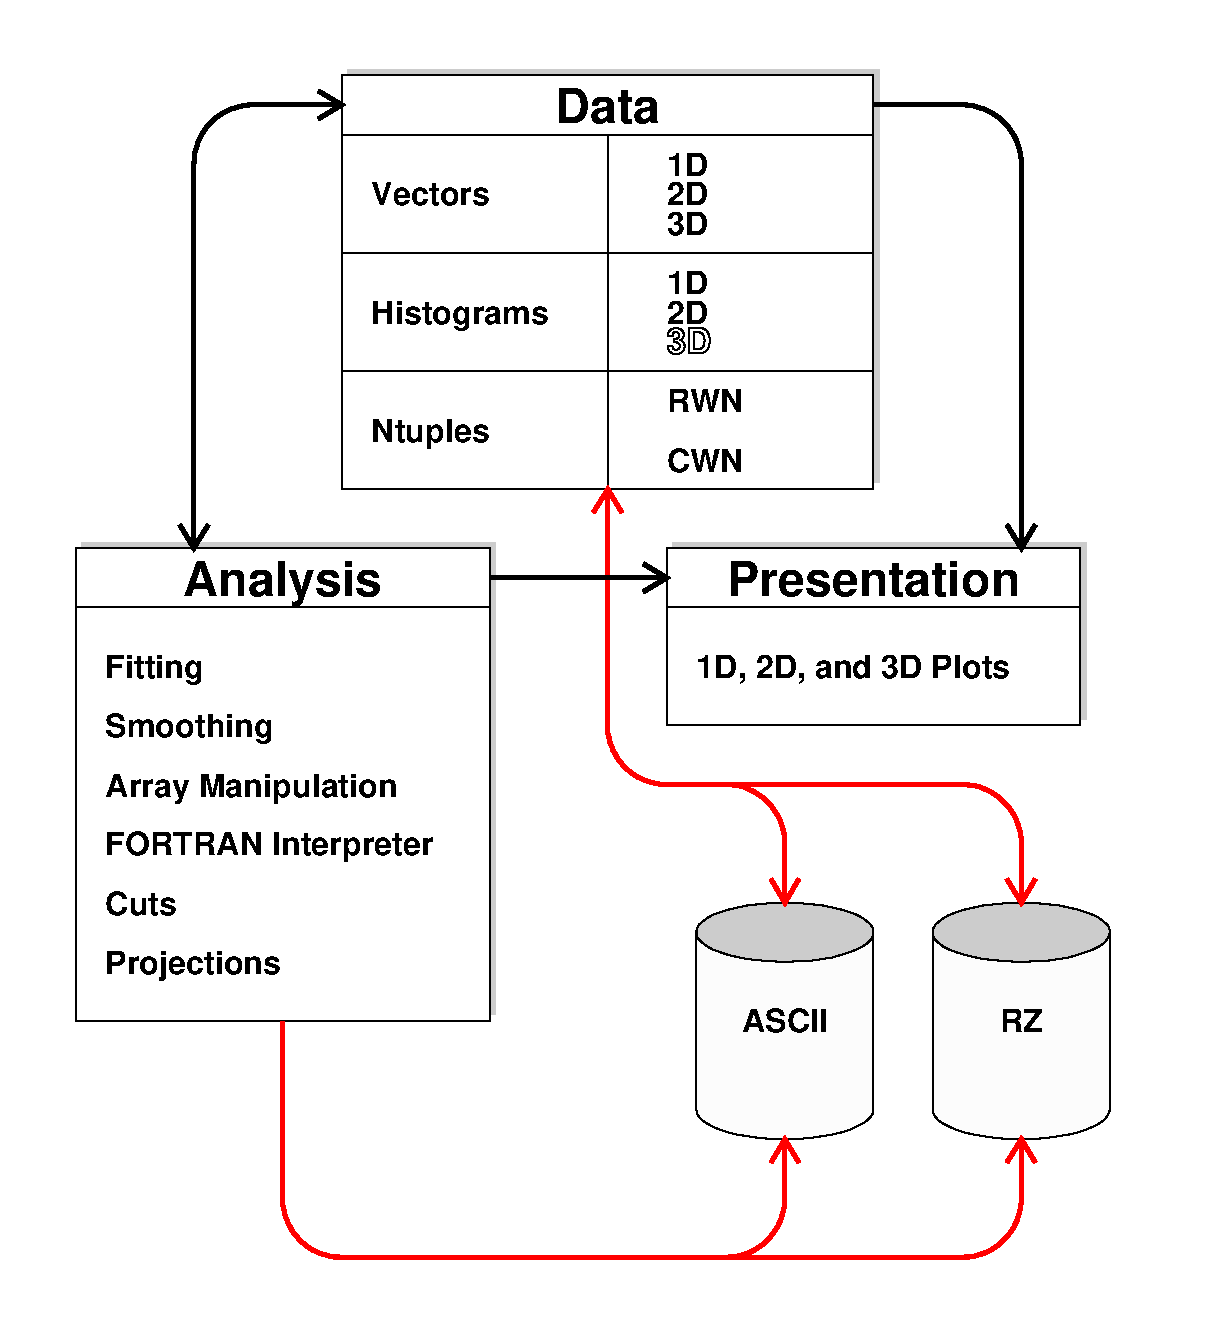
\epsfig{file=pawtut01.eps,height=.5\linewidth}}
\end{center}
\caption{PAW's fundamental ``data'' objects}
\label{fig:pawobjects}
\end{figure}

\subsection*{Objects:}

\begin{itemize}
\item {\bf 1D Histograms.}  
\index{histogram}
\index{histogram!1D}
      A histogram is the basic statistical analysis tool of PAW. Histograms are
      created (``booked'') by choosing the basic characteristics of their bins,
      variables, and perhaps customized display parameters; numbers are entered
      into the histogram bins from an Ntuple (the histogram is ``filled'') by 
      selecting the desired events, weights, and variable transformations to be
      used while counts are accumulated in the bins. Functional forms are 
      frequently fit to the resulting histograms and stored with them. Thus a 
      fit as an object is normally associated directly with a histogram, 
      although it may be considered separately.
\item {\bf 2D Histograms.}  
\index{histogram!2D}
      2D (and higher-dimensional) histograms are logical generalizations of 1D
      histograms. 2D histograms, for example, are viewable as the result of 
      counting the points in a the sections of a rectangular grid overlaid on 
      a scatter plot of two variables. Higher-dimensional histograms can also 
      be fitted, and support for associating the results of a fit to a 
      higher-dimensional histogram is currently being incorporated in PAW.
\item {\bf Ntuples.}  
\index{Ntuple}
      An Ntuple is the basic type of data used in PAW. It consists of a list of
      identical data structures, one for each event. Typically, an Ntuple is 
      made available to PAW by opening a HBOOK file; this file, as created by 
      HBOOK, contains one or more Ntuples and possibly also directories, which
      may store a hierarchy of Ntuples and histograms. A storage area for an 
      Ntuple may be created directly using \Ucom{NTUPLE/CREATE}; data may then
      be stored in the allocated space using the \Ucom{NTUPLE/LOOP} or 
     \Ucom{NTUPLE/READ} commands. Other commands merge Ntuples into larger 
      Ntuples, project vector functions of the Ntuple variables into histograms,
      and plot selected subsets of events.
\item {\bf Cuts.}  
\index{cut}
      A cut is a Boolean function of Ntuple variables. Cuts are used to select
      subsets of events in an Ntuple when creating histograms and ploting 
      variables.
\item {\bf Masks.}  
\index{mask}
      Masks are separate files that are logically identical to a set of boolean 
      variables added on the end of an Ntuple's data structure. A mask is 
      constructed using the Boolean result of applying a cut to an event set.
      A mask is useful only for efficiency; the effect of a mask is identical 
      to that of the cut that produced it.
\item {\bf Vectors.}  
\index{vector}
      PAW provides the facilities to store vectors of integer or real data. 
      These vectors, or rather arrays with up to 3 index dimensions, can be 
      manipulated with a set of dedicated commands. Furthermore they are 
      interfaced to the array manipulation package SIGMA and to the Fortran 
      interpreter COMIS. They provide a convenient and easy way to analyse 
      small data sets stored in ASCII files.
\item {\bf PostScript (meta)files.}  
\index{metafile}
      PostScript format (meta)files are especially useful because they can be 
      directly printed on most printers; furthermore, the printed quality of 
      graphics objects such as fonts can be of much higher quality than the 
      original screen image.
\item {\bf Pictures.}  
\index{picture}
      A {\it picture\/} is an exact copy of the screen image, and so its
      storage and redisplay time are independent of complexity. Pictures are 
      also intensively used for object picking in the Motif version of PAW.
\item {\bf ZEBRA(RZ) Logical Directories.}  
\index{directory!ZEBRA}
      In a single PAW session, the user may work simultaneously with many 
      Ntuples, histograms, and hierarchies of Ntuple and histograms. However, 
      this is not accomplished using the native operating system's file handler.
      Instead, the user works with a set of objects that are {\it similar\/} to
      a file system, but are instead managed by the ZEBRA RZ package. This can
      be somewhat confusing because a single operating system file created by 
      RZ can contain an entire hierarchy of ZEBRA logical directories; 
      furthermore, sections of internal memory can also be organized as ZEBRA 
      logical directories to receive newly-created PAW objects that are not 
      written to files. A set of commands \Ucom{CDIR}, \Ucom{LDIR}, and 
      \Ucom{MDIR} are the basic utilities for walking through a set of ZEBRA 
      logical directories of PAW objects; Each set of directories contained in
      an actual file corresponds to a logical unit number, and the root of the
      tree is usually of the form \texttt{//LUNx};  the PAW objects and logical
      directories stored in internal memory have the root \texttt{//PAWC}.
\index{Macros}
\index{macro}
      A macro is a set of command lines stored in a file, which can be created 
      or modified with any text editor. In addition to all the PAW commands, 
      special macro flow control statements are also available.
\item {\bf Operating System File Directories.}  
\index{operating system}
      Many different ZEBRA files, some with logically equivalent Ntuples and 
      histograms, can be arranged in the user's operating system file 
      directories. Thus one must also keep clearly in mind the operating system
      file directories and their correspondence to the ZEBRA logical directories
      containing data that one wishes to work with.  In many ways, the operating
      system file system is also a type of ``object'' that forms an essential 
      part of the user's mental picture of the system.
\end{itemize}
 

\begin{figure}
\centering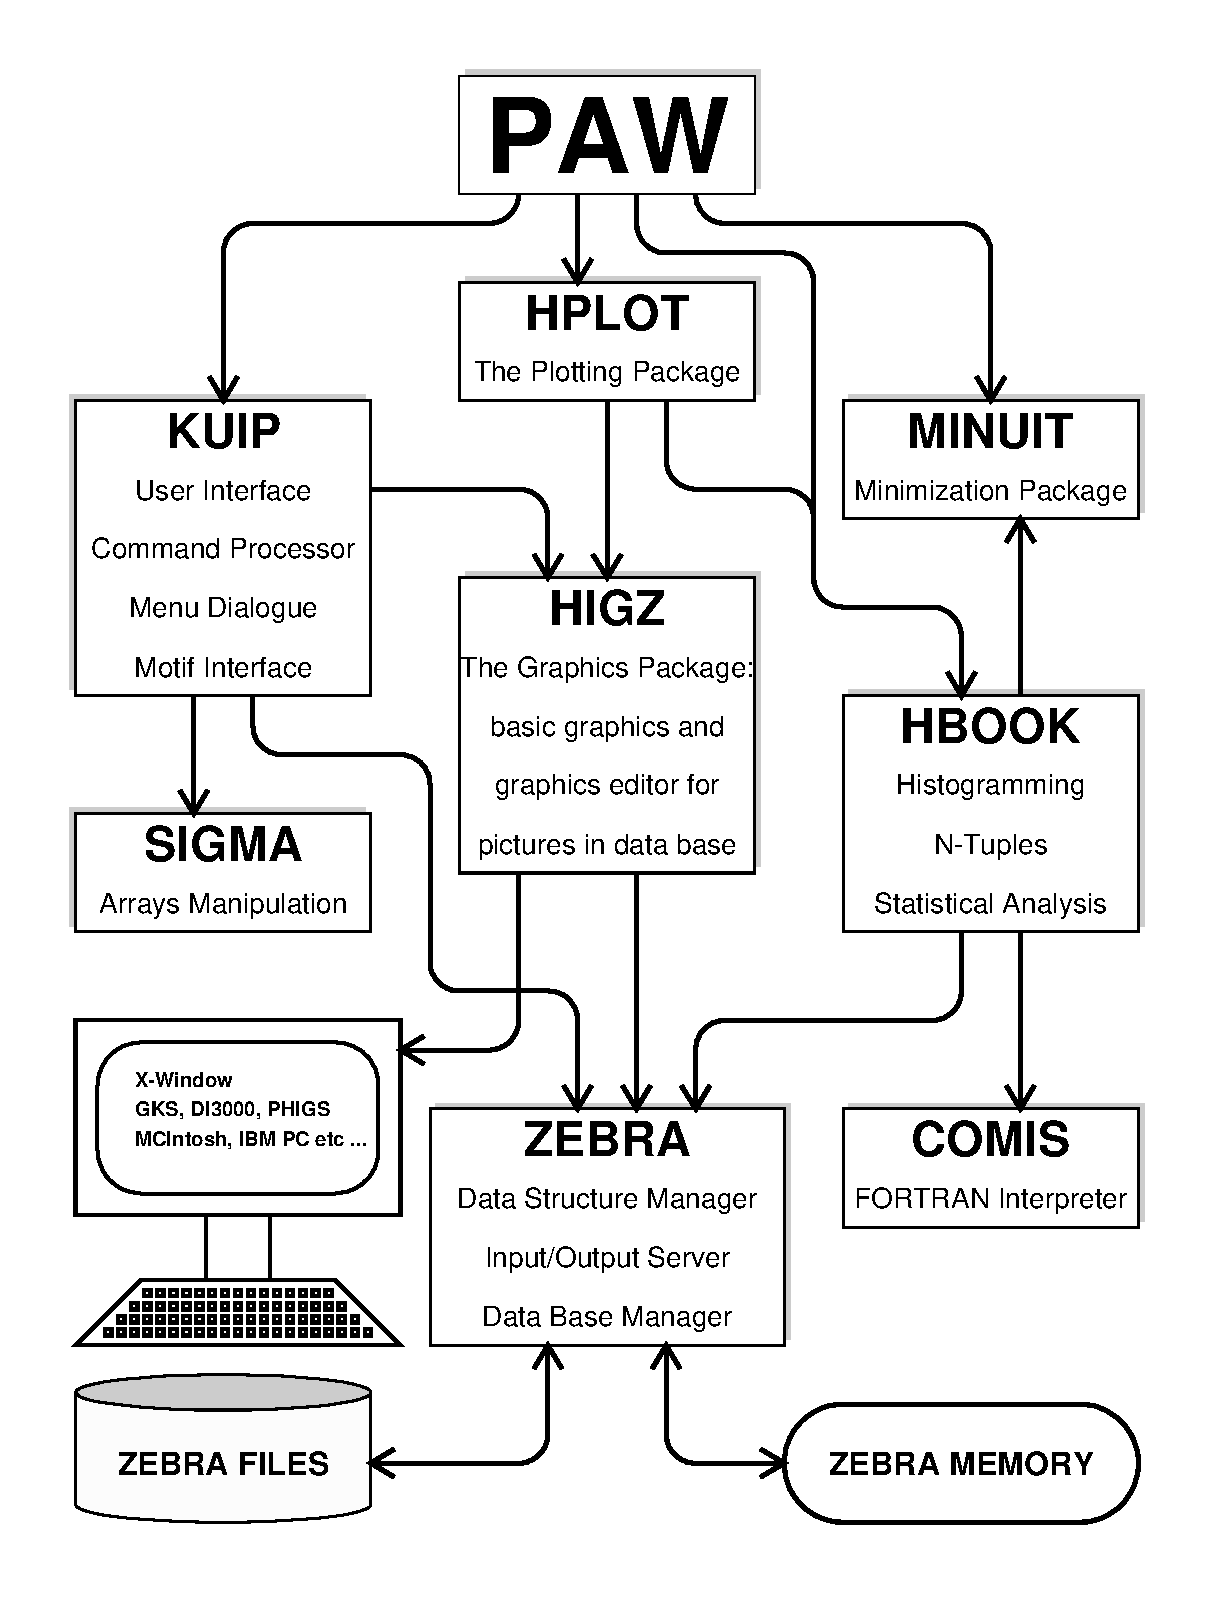
\includegraphics[width=.5\textwidth]{pawtut00.eps}
\caption{PAW and its components}
\label{fig:PAWcomp}
\end{figure}

\section{The Component Subsystems of PAW}
\label{sec:pawstructure}
\index{structure of PAW}
\index{PAW!structure}

The PAW system combines different tools and packages, which
can also be used independently and some of which have already
a long history behind them (e.g. HBOOK and
HPLOT, SIGMA, COMIS, MINUIT).
Figure \ref{fig:PAWcomp} shows the various components of PAW.
\index{components!of PAW}

\subsection{KUIP - The user interface package}
\index{KUIP}
\index{command!definition file (CDF)}
\index{CDF Command Definition File}
\index{alias}
\index{abbreviation}
\index{macro}
\index{dialogue style}
\index{default setting}
\index{history file}
 
The purpose of KUIP
({\bf K}it for a {\bf U}ser
{\bf I}nterface {\bf P}ackage) is to handle
the dialogue between the user and the application program (PAW
in our case). It
parses the commands input into the system, verifies them for
correctness and then hands over control to the relevant action
routines.
 
\index{command!abbreviation}
Commands are grouped in a tree structure and they can be
{\bf abbreviated} to their shortest unambiguous
form. If an ambiguous command is typed, then KUIP responds by showing
all the possibilities.
\index{alias}
{\bf Aliases} allow the user to abbreviate part or the whole
of commonly used command and parameters.
A sequence of PAW commands can be stored in a text file and, combined
with flow control statements, form a powerful {\bf macro} facility.
\index{macro!parameter}
\index{parameter}
With the help of {\bf parameters},
whose values can be passed to the macros, general and adaptable
task solving procedures can be developed.
 
\index{style of dialogue}
\index{dialogue!style}
 The user has the choice between different dialogue styles ranging from
the conventional command line interface to a high-level windowed environment
based on OSF/Motif \index{Motif}.
In order to save typing, {\bf default values},
providing reasonable settings, can be used for most
\index{history file}
parameters of a command. A {\bf history file},
containing the {\tt\underline{n}} most recently entered
commands, is automatically kept by KUIP
and can be inspected, copied or re-entered at any time.
The history file of the last PAW session is also kept on disk.

\subsection{HBOOK and HPLOT - The histograming and plotting packages}
\index{HBOOK}
\index{HPLOT}

HBOOK and its graphics interface
HPLOT are libraries of FORTRAN callable
subroutines which have been
in use for many years.
They provide the following functionality:

\begin{UL}
\item One- and two-dimensional histograms and Ntuples
\item Projections and slices of two-dimensional histograms and Ntuples
\item Complete control (input and output) of the histogram contents
\item Operations and comparison of histograms
\item Minimization and parameterization tools
\item Random number generation
\item Histograms and Ntuples structured in memory (directories)
\item Histograms and Ntuples saved onto direct access ZEBRA files
\item Wide range of graphics options:
\begin{UL}
\item Contour histograms, bar chart, shaded histograms, error bars, colour
\item Smoothed curves and surfaces
\item Scatter, lego, contour and surface plots
\item Automatic windowing
\item Graphics input
\end{UL}
\end{UL}

\subsection{HIGZ - The graphics interface package}
\index{HIGZ}

A {\bf H}igh level
{\bf I}nterface to {\bf G}raphics and {\bf Z}EBRA
(HIGZ) has been developed within the PAW project. This package is
a layer between the application program (e.g. PAW/HPLOT) and the basic
graphics package (e.g. X11) on a given system. Its basic aims are:

\begin{UL}
\item Full transportability of the picture data base.
\item Easy manipulation of the picture elements.
\item Compactness of the data to be transported and accessibility
      of the pictures in direct access mode.
\item Independence of the underlying basic graphics package.
      Presently HIGZ is interfaced with several GKS packages,
      X- Windows (X11), PHIGS, Mac, PC's graphic systems, 
      GL (Silicon Graphics), GDDM (IBM),
      GPR (Apollo) as well as with the DI3000 system. Note that some of these
      graphics systems are now obsolete. PAW is now mainly used in its X11 
      version.
\index{GKS}
\index{X windows}
\index{GL (Silicon Graphics)}
\index{GPR (Apollo)}
\index{GMR3D (Apollo)}
\index{GDDM (IBM)}
\index{DI3000}
\end{UL}

These requirements have been incorporated into HIGZ by exploiting
the data management system ZEBRA.
 
HIGZ does not introduce new basic graphics features, but introduces
some macroprimitives for frequently used functions
(e.g. arcs, axes, boxes, pie-charts, tables). The system
provides the following features:

\begin{UL}
\item Basic graphics functions: basic primitives, attributes, space definition.
\item Higher-level macroprimitives.
\item Data structure management using an interface to the ZEBRA system.
\item Interactive picture editing.
\end{UL}

These features, which are available simultaneously, are
particularly useful during
an interactive session, as the user is able to
``replay'' and edit previously created pictures, without the need to re-run
\index{replay}
the application program. 
A direct interface to PostScript is also
available.

\subsection{ZEBRA - The data structure management system}
\index{ZEBRA}

The data structure management package ZEBRA
was developed at CERN in order to overcome the lack of dynamic
data structure facilities in FORTRAN, the favourite computer language
in high energy physics. It implements the {\bf dynamic
creation and modification} of data structures at execution time
and their transport
to and from external media on the same or different computers, memory
to memory, to disk or over the network, at an
{\bf insignificant cost} in terms of execution-time overheads.
 
\index{input/output}
\index{native input/output}
\index{exchange input/output}
\index{RZ file}
ZEBRA manages any type of structure, but specifically
supports linear structures (lists) and trees.
ZEBRA input/output is either of a sequential or direct access type.
Two data representations,
{\bf native} (no data conversion when transferred to/from the
external medium) and {\bf exchange} (a conversion to an
interchange format is made), allow data to be transported between
computers of the same and of different architectures.
The direct access package {\bf RZ} can be used
to manage hierarchical data bases. In PAW this facility is exploited
to store histograms, Ntuples and pictures in a hierarchical direct access
directory structure.

\subsection{MINUIT - Function minimization and error analysis}
\index{MINUIT}
\index{fit}
\index{statistic!analysis}
\index{minimisation}
\index{chisquare}
\index{correlation}
 
MINUIT is a tool to find the {\bf minima of a
multi-parameter function} and
analyse the {\bf shape around the minimum}. It can be used for
{\bf statistical analysis} of
curve fitting, working on a \(\chi^2\) or log-likelihood function,
to compute the {\bf best fit} parameter values, their uncertainties and
correlations. {\bf Guidance} can be provided in order to find the
correct solution, parameters can be kept fixed and data points
can be easily added or removed from the fit. An interactive Motif based
interface is in preparation.

\subsection{COMIS - The FORTRAN interpreter}
\index{COMIS}

The COMIS interpreter allows the user to execute interactively
a set of FORTRAN routines in interpretive mode.
The interpreter implements a large subset of the complete FORTRAN
language. It is an extremely important tool because
it allows the user
to specify his own complex data analysis procedures, for example
selection criteria or a minimisation function.

\subsection{SIGMA - The array manipulation language}
\index{SIGMA}

A scientific computing programming language SIGMA
({\bf S}ystem for {\bf I}nteractive
{\bf G}raphical {\bf M}athe\-ma\-tical
{\bf A}pplications),
which was designed essentially for mathematicians and
theoretical physicists is integrated into PAW.  Its main characteristics are:

\begin{UL}
\item The basic data units are scalars and one or more dimensional
      rectangular arrays, which are automatically handled.
\item The computational operators resemble those of FORTRAN.
\end{UL}

\section{A PAW Glossary}

\subsection*{Data Analysis Terminology}


\begin{DL}{MMMMM}
\item[DST]       A ``Data Summary Tape'' is one basic form of  output from
                 a typical physics experiment.  A DST is generally not used
                 directly by PAW, but is analyzed by customized user programs
                 to produce Ntuple files, which PAW can read directly.
\index{DST}
\index{DST!Data Summary Tape}
\item[Ntuple]    A list of identical data structures, each typically 
                 corresponding to a single experimental event. The data 
                 structures
                 themselves frequently consist of a row of numbers, so that
                 many Ntuples may be viewed as
                 two-dimensional arrays of data variables, with one
                 index of the array describing the position of the data
                 structure in the list (i.e., the row or event number),
                 and the other index referring to the position of the data
                 variable in the row (i.e., the column or variable number).
                 A meaningful name is customarily assigned to each column
                 that describes the variable contained in that column for each
                 event.  
\index{Ntuple}
\item[Event]     A single instance of a set of data  or experimental measurements,
                 usually consisting of a sequence of variables or structures of
                 variables resulting from a partial analysis of the raw data.
                 In PAW applications, one typically examines the statistical
                 characteristics of large sequences of similar events.
\index{event}
\item[Variable]  One of a user-defined set of named values associated with a single
                 event in an Ntuple.
                 For example,
                 the \((x,\,y,\,z)\) values of a momentum vector could each
                 be variables for a given event.  Variables are typically
                 useful experimental quantities that are stored in an
                 Ntuple;  they are used in algebraic formulas
                 to define boolean cut criteria
                 or other dependent variables that are
                 relevant to the analysis.
\item[Cut]       A  boolean-valued function of the variables of a given event.
                 Such functions allow the user to specify that only  events
                 meeting certain criteria are to be included in a given distribution.
\index{cut}
\item[Mask]      A set of columns of zeros and ones that is identical in form
                 to a new set of Ntuple variables.  A mask is typically
                 used to save the results of applying a set of cuts to a large
                 set of events so that
                 time-consuming selection computations are not repeated needlessly.
\index{mask}
\item[Function]  Sequence of one or more statements with a FORTRAN-like syntax
                 entered on the command line or via an external file.
\index{function}
\end{DL}

\subsection*{Statistical Analysis Terminology}

\begin{DL}{MMMMM}
\item[Histogram] A one- or two-dimensional array of data, generated
                 by HBOOK in batch or in a PAW session. Histograms are (implicitly or
                 explicitly) declared (booked);
                 they can be filled by explicit entry of data
                 or can be derived from other histograms. The information stored
                 with a histogram includes a title, binning and packing definitions,
                 bin contents and errors, statistic values, possibly an
                 associated function vector, and output attributes.
                 Some of these items are optional.
                 The ensemble of this information constitutes an {\bf histogram}.
\index{histogram}
\index{histogram!booking}
\item[Booking]   The operation of declaring (creating) an histogram.
\index{book histogram}
\item[Filling]   The operation of entering data values into a given histogram.
\index{fill!histogram}
\index{histogram!filling}
\item[Fitting]   Least squares and maximum likelihood fits of
                 parametric functions to histograms and vectors.
\index{fit}
\item[Projection]The operation of projecting two-dimensional
                 distributions onto either or both axes.
\index{projection}
\item[Band]      A band is a projection onto the X (or Y) axis
                 restricted to an interval
                 along the other Y (or X) axis.
\index{band}
\item[Slice]     A slice is a projection onto the X (or Y) 
                 axis restricted to one bin
                 along the other Y (or X) axis.
                 Hence a slice is a special case of a band, with
                 the interval limited to one bin.
\index{slice}
\item[Weight]    PAW allows the user to include a
                 multiplicative statistical bias for each event which is a scalar
                 function of the available variables.  This permits the user to
                 correct for known statistical biases in the data when making
                 histograms of event distributions.
\end{DL}

\subsection*{KUIP/ZEBRA User Environment Terminology}

\begin{DL}{MMMMM}
\item[Macro]     A text file containing a set commands 
                 and logical constructs to control the flow of execution. 
                 Parameters can be supplied when calling a macro.
\index{macro}
\item[Vector]    The equivalent of a FORTRAN array supporting 
                 up to three dimensions.
                 The elements of a vector can be stored using a real or an
                 integer representation;
                 they can be entered interactively on a terminal or read
                 from an external file.
\index{vector}
\item[Logical Directory\ ]
                 The ZEBRA data storage system resembles a file system organized
                 as logical directories.  PAW maintains
                 a global variable corresponding to the ``current directory'' where
                 PAW applications will look for PAW objects such as histograms.
                 The ZEBRA directory structure is a tree, and user functions permit
                 the ``current directory'' to be set anywhere in the current tree,
                 as well as creating new ``directories'' where the results
                 of PAW actions can be stored.  A special
                 directory called \texttt{//PAWC} corresponds to a memory-resident
                 branch of this virtual file system.  ZEBRA files may be written
                 to the operating system file system, but entire hierarchies of
                 ZEBRA directories typically are contained in a single binary operating
                 system file.
\end{DL}

\subsection*{Graphics Production Terminology}

\begin{DL}{MMMMM}
\item[Metafile]  A file containing graphical information
                 stored in a device independent format,
                 which can be replayed on various types of output devices.
                 (e.g. PostScript).
\index{metafile}
\item[Picture]   A graphics object composed of graphics primitives 
                 and attributes.
                 Pictures are generated by
                 the HIGZ graphics interface and they can be stored in a picture
                 direct-access database, built with the RZ-package of the
                 data structure manager ZEBRA.
\index{picture}
\index{PostScript}
\item[PostScript]
                 A high level page description language permitting the description of complex
                 text and graphics using only text commands.  Using PostScript
                 representations of graphics makes it possible to create graphics
                 files that can be exchanged with other users and printed on
                 a wide variety of printers without regard to the computer system
                 upon which the graphics were produced.  Any graphics display
                 produced by PAW can be expressed in terms of PostScript, written
                 to a file, and printed.
\end{DL}
 
\endinput
